\subsection{Mesa de posicionamento}

% SLIDE DE MESA DE POSICIONAMENTO
\begin{frame}
\frametitle{Mesa de posicionamento}

Podem ser classificadas em dois tipos com relação a sua transmissão: as mesas acionadas por fusos e por correias sincronizadas.

\begin{figure}
\centering
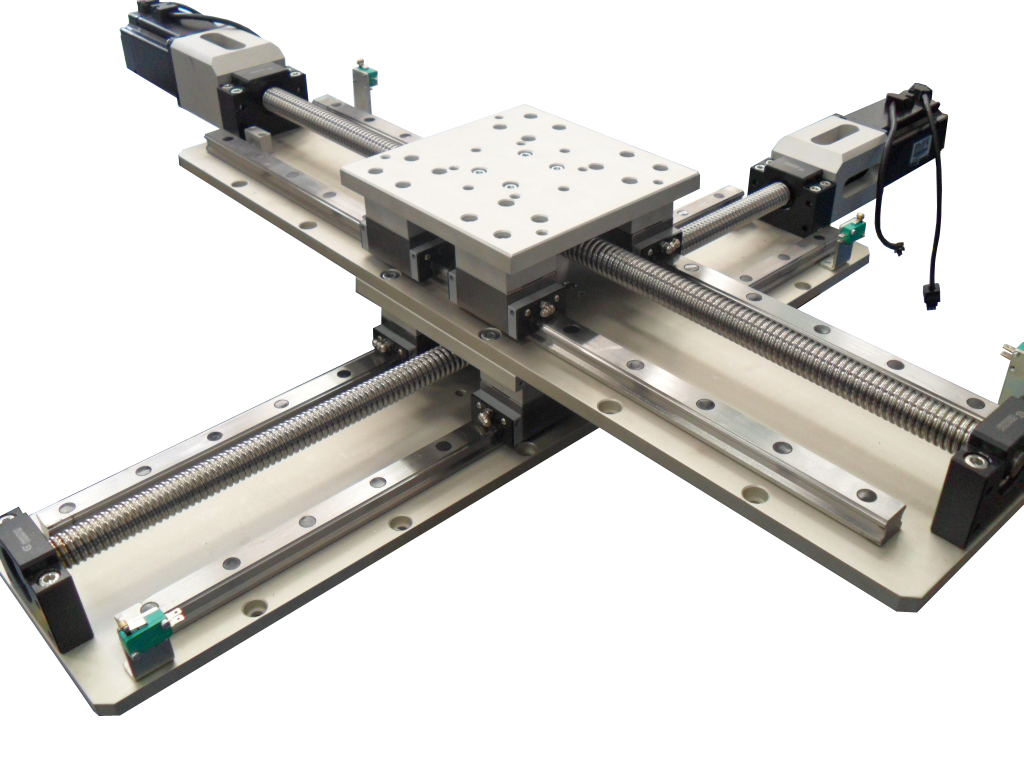
\includegraphics[scale = 0.12]{figs/mfuso}
\end{figure}

\begin{figure}
\centering
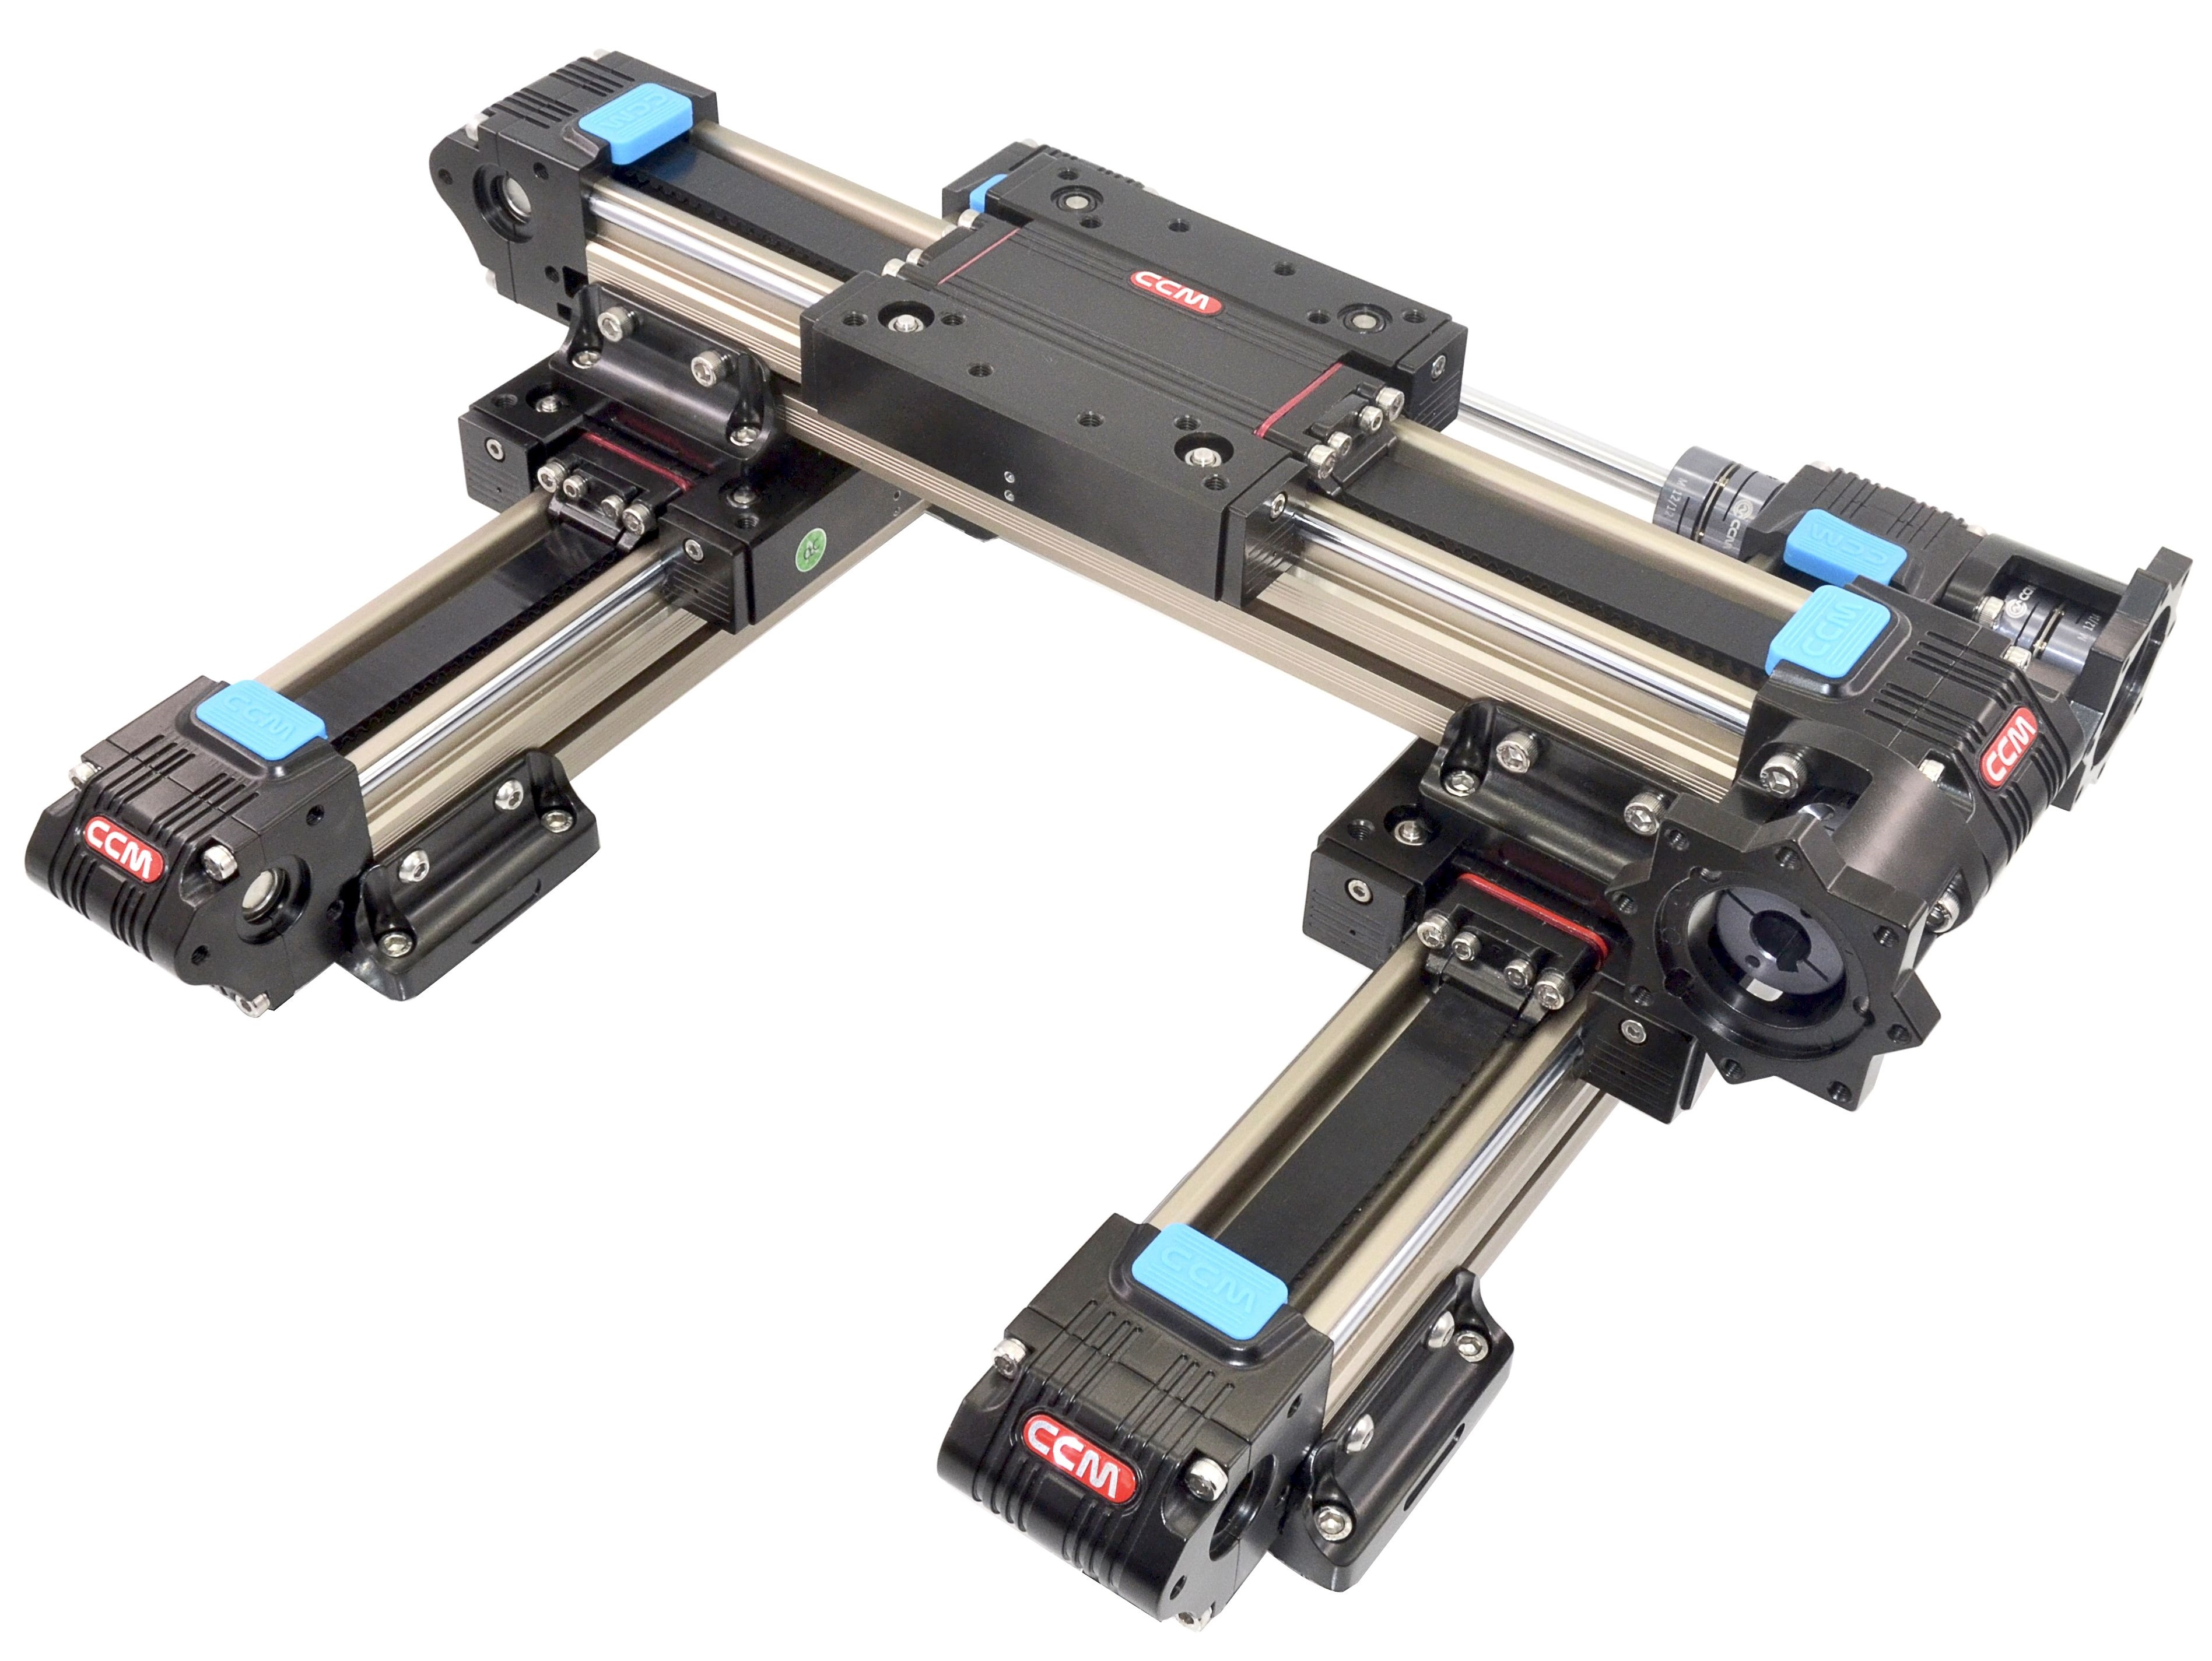
\includegraphics[scale = 0.03]{figs/mcorreia}
\end{figure}
    
\end{frame}
    
% SLIDE DE MESA DE POSICIONAMENTO
\begin{frame}
\frametitle{Mesa de posicionamento}

Outro componente importante é o acionador, que pode ser um motor de passo ou um servomotor. 

Os motores de passo são máquinas utilizadas em aplicações de um alto grau de precisão no movimento em passos fixos, referentes a uma fração de ângulo. 

\begin{figure}
\centering
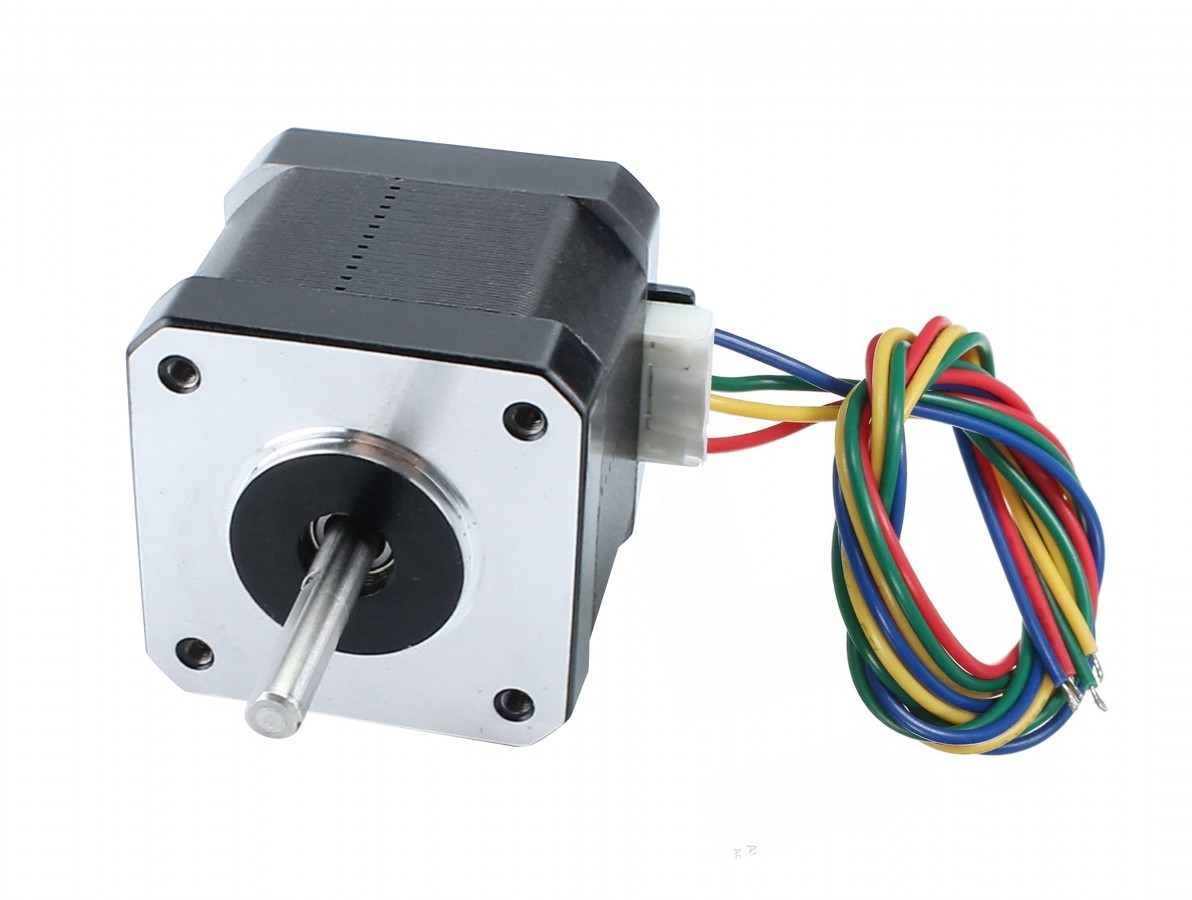
\includegraphics[scale = 0.07]{figs/motordepassoex}
\end{figure}

\begin{figure}
\centering
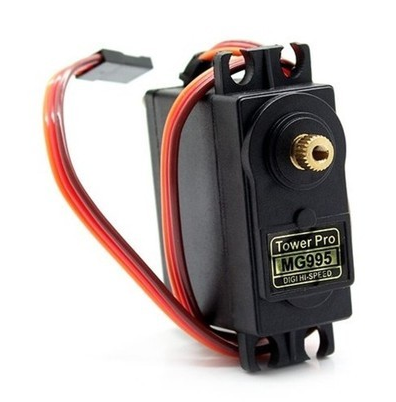
\includegraphics[scale = 0.13]{figs/servomotorex}
\end{figure}
    
\end{frame}
